\documentclass[12pt,twoside,a4paper]{article}

\textwidth 17cm \textheight 25cm \evensidemargin 0cm
\oddsidemargin 0cm \topmargin -2.5cm
\parindent 0pt
%\parskip \bigskipamount

\usepackage{graphicx}
\usepackage[dutch]{babel}
\usepackage{amssymb,amsthm,amsmath}
\usepackage[utf8]{inputenc}
\usepackage{nopageno}
\usepackage{pdfpages}
\usepackage{enumerate}
\usepackage{caption}
\usepackage{wrapfig}
\usepackage{pgf,tikz}
\usepackage{color}
\usetikzlibrary{arrows}
\usetikzlibrary{patterns}
\usepackage{fancyhdr}
\pagestyle{fancy}
\usepackage[version=3]{mhchem}
\usepackage{multicol}
\usepackage{fix-cm}
\usepackage{setspace}
\usepackage{mhchem}
\usepackage{xhfill}
\usepackage{parskip}
\usepackage{cancel}
\usepackage{mdframed}
\usepackage{url}

\newcommand{\todo}[1]{{\color{red} TODO: #1}}

\newcommand{\degree}{\ensuremath{^\circ}}
\newcommand\rad{\qopname\relax o{\mathrm{rad}}}

\newcommand\ggd{\qopname\relax o{\mathrm{ggd}}}

\def\LRA{\Leftrightarrow}%\mkern40mu}

\newcommand{\zrmbox}{\framebox{\phantom{EXE}}\phantom{X}}
\newcommand{\zrm}[1]{\framebox{#1}}

% environment oefening:
% houdt een teller bij die de oefeningen nummert, probeert ook de oefening op één pagina te houden
\newcounter{noefening}
\setcounter{noefening}{0}
\newenvironment{oefening}
{
  \stepcounter{noefening}
  \pagebreak[0]
  \begin{minipage}{\textwidth}
  \vspace*{0.7cm}{\large\bf Oefening \arabic{noefening}}
}{%
  \end{minipage}
}

\usepackage{calc}

% vraag
\reversemarginpar
\newcounter{punten}
\setcounter{punten}{0}
\newcounter{nvraag}
\setcounter{nvraag}{1}
\newlength{\puntwidth}
\newlength{\boxwidth}
\newcommand{\vraag}[1]{
\settowidth{\puntwidth}{\Large{#1}}
\setlength{\boxwidth}{1.5cm}
\addtolength{\boxwidth}{-\puntwidth}
{\large\bf Vraag \arabic{nvraag} \addtocounter{nvraag}{1}}\vspace*{-0.5cm}
{\marginpar{\color{lightgray}\fbox{\parbox{1.5cm}{\vspace*{1cm}\hspace*{\boxwidth}{\Large{#1}}}}}
\vspace*{0.5cm}}
\addtocounter{punten}{#1}}

% arulefill
\newcommand\arulefill[1][]{
  \ifstrempty{#1}{
    \leavevmode{
      \xrfill[-5pt]{0.3pt}[lightgray]
      \endgraf
    }
    \vspace*{0.2cm}
  }{
    \leavevmode{
      \xrfill[-5pt]{0.3pt}[lightgray]
      \endgraf
      \vspace*{0.2cm}
    }
    \foreach \n in {1,...,#1}{
      \leavevmode{
        \xrfill[-5pt]{0.3pt}[lightgray]
        \endgraf
        \vspace*{0.2cm}
      }
    }
  }
}
% \arules{n}
\newcommand{\arules}[1]{
\mbox{}
\color{lightgray}
%\vspace*{0.05cm}
\foreach \n in {1,...,#1}{
  \vspace*{0.75cm}
  \hrule height 0.3pt\hfill
}\color{black}\vspace*{0.2cm}}

% \arule{x}
\newcommand{\arule}[1]{
\color{lightgray}{\raisebox{-0.1cm}{\rule[-0.05cm]{#1}{0.3pt}}}\color{black}
}

% \abox{y}
\newcommand{\abox}[1]{
\fbox{
\begin{minipage}{\textwidth- 4\fboxsep}
\hspace*{\textwidth}\vspace{#1}
\end{minipage}
}
}

\newcommand{\ruitjes}[1]{
\definecolor{cqcqcq}{rgb}{0.85,0.85,0.85}
\hspace*{-2.5cm}
\begin{tikzpicture}[scale=1.04,line cap=round,line join=round,>=triangle 45,x=1.0cm,y=1.0cm]
\draw [color=cqcqcq, xstep=0.5cm, ystep=0.5cm] (0,-#1) grid (20.5,0);
\end{tikzpicture}
}


\newcommand{\assenstelsel}[5][1]{
\definecolor{cqcqcq}{rgb}{0.65,0.65,0.65}
\begin{tikzpicture}[scale=#1,line cap=round,line join=round,>=triangle 45,x=1.0cm,y=1.0cm]
\draw [color=cqcqcq,dash pattern=on 1pt off 1pt, xstep=1.0cm,ystep=1.0cm] (#2,#4) grid (#3,#5);
\draw[->,color=black] (#2,0) -- (#3,0);
\draw[shift={(1,0)},color=black] (0pt,2pt) -- (0pt,-2pt) node[below] {\footnotesize $1$};
\draw[color=black] (#3.25,0.07) node [anchor=south west] { x};
\draw[->,color=black] (0,#4) -- (0,#5);
\draw[shift={(0,1)},color=black] (2pt,0pt) -- (-2pt,0pt) node[left] {\footnotesize $1$};
\draw[color=black] (0.09,#5.25) node [anchor=west] { y};
\draw[color=black] (0pt,-10pt) node[right] {\footnotesize $0$};
\end{tikzpicture}
}

\newcommand{\getallenas}[3][1]{
\definecolor{cqcqcq}{rgb}{0.65,0.65,0.65}
\begin{tikzpicture}[scale=#1,line cap=round,line join=round,>=triangle 45,x=1.0cm,y=1.0cm]
\draw [color=cqcqcq,dash pattern=on 1pt off 1pt, xstep=1.0cm,ystep=1.0cm] (#2,-0.2) grid (#3,0.2);
\draw[->,color=black] (#2.25,0) -- (#3.5,0);
\draw[shift={(0,0)},color=black] (0pt,2pt) -- (0pt,-2pt) node[below] {\footnotesize $0$};
\draw[shift={(1,0)},color=black] (0pt,2pt) -- (0pt,-2pt) node[below] {\footnotesize $1$};
\draw[color=black] (#3.25,0.07) node [anchor=south west] {$\mathbb{R}$};
\end{tikzpicture}
}

\newcommand{\visgraad}[1]{\begin{tabular}{p{0.5cm}|p{#1}}&\\\hline\\\end{tabular}}

\newcommand{\tekenschema}[2]{\begin{tabular}{p{0.5cm}|p{#1}}&\\\hline\\[#2]\end{tabular}}

% schema van Horner
\newcommand{\schemahorner}{
\begin{tabular}{p{0.5cm}|p{7cm}}
&\\[1.5cm]
\hline\\
\end{tabular}}

% geef tabular iets meer ruimte
\setlength{\tabcolsep}{14pt}
\renewcommand{\arraystretch}{1.5}

\newcommand{\toets}[3]{
\thispagestyle{plain}
\vspace*{-2.5cm}
\begin{tikzpicture}[remember picture, overlay]
    \node [shift={(15.25 cm,-1.6cm)}] {%
        \includegraphics[width=1.8cm]{/home/ppareit/kaa1415/logokaavelgem.png}%
    };%
\end{tikzpicture}

\begin{tabular}{|llc|c|}
\hline
\vspace*{-0.5cm}
&&&\\
Naam & \arule{4cm} & {\Large\bf KA AVELGEM} & \\
\vspace*{-0.75cm}
&&&\\
Klas & \arule{4cm} & {\Large\bf 20...-...-...} & \\
\hline
\vspace*{-0.75cm}
&&&\\
Toets & {\bf #2} & {\large\bf #1} & Beoordeling\\
\vspace*{-0.75cm}
&&&\\
Onderwerp & \multicolumn{2}{l|}{\bf #3} &\\
\hline
\end{tabular}
}

\newcommand{\oefeningen}[1]{

\fancyhead[LE, RO]{\vspace{0.5cm} #1}
%\thispagestyle{plain}

{\bf \Large \centering Oefeningen: #1}

}

\raggedbottom

\newcommand\dom{\qopname\relax o{\mathrm{dom}}}
\newcommand\ber{\qopname\relax o{\mathrm{ber}}}

\newcommand\mC{\qopname\relax o{\mathrm{mC}}}
\newcommand\uC{\qopname\relax o{\mathrm{{\mu}C}}}
\newcommand\C{\qopname\relax o{\mathrm{C}}}

\newcommand\W{\qopname\relax o{\mathrm{W}}}
\newcommand\kW{\qopname\relax o{\mathrm{kW}}}
\newcommand\kWh{\qopname\relax o{\mathrm{kWh}}}


\newcommand\V{\qopname\relax o{\mathrm{V}}}
\newcommand\ohm{\qopname\relax o{\mathrm{\Omega}}}
\newcommand\kohm{\qopname\relax o{\mathrm{k\Omega}}}


\newcommand\N{\qopname\relax o{\mathrm{N}}}

\newcommand\Nperkg{\qopname\relax o{\mathrm{N/kg}}}

\newcommand\Nperm{\qopname\relax o{\mathrm{N/m}}}

\newcommand\gpermol{\qopname\relax o{\mathrm{g/mol}}}


\newcommand\kgperm{\qopname\relax o{\mathrm{kg/m}}}
\newcommand\kgperdm{\qopname\relax o{\mathrm{kg/dm}}}
\newcommand\gpercm{\qopname\relax o{\mathrm{g/cm}}}
\newcommand\gperml{\qopname\relax o{\mathrm{g/ml}}}


\newcommand{\mA}{\;\mbox{mA}}
\newcommand{\A}{\;\mbox{A}}
\newcommand{\MA}{\;\mbox{MA}}

\newcommand{\us}{\;\mu\mbox{s}}
\newcommand\s{\qopname\relax o{\mathrm{s}}}

\newcommand\h{\qopname\relax o{\mathrm{h}}}

\newcommand{\mpers}{\;\mbox{m/s}}
\newcommand{\kmperh}{\;\mbox{km/h}}
\newcommand{\kmpermin}{\;\mbox{km/min}}
\newcommand{\kmpers}{\;\mbox{km/s}}

\newcommand{\mph}{\;\mbox{mph}}

\newcommand{\Hz}{\;\mbox{Hz}}

\newcommand\Gm{\qopname\relax o{\mathrm{Gm}}}
\newcommand\Mm{\qopname\relax o{\mathrm{Mm}}}
\newcommand\km{\qopname\relax o{\mathrm{km}}}
\newcommand\hm{\qopname\relax o{\mathrm{hm}}}
\newcommand\dam{\qopname\relax o{\mathrm{dam}}}
\newcommand\m{\qopname\relax o{\mathrm{m}}}
\newcommand\dm{\qopname\relax o{\mathrm{dm}}}
\newcommand\cm{\qopname\relax o{\mathrm{cm}}}
\newcommand\mm{\qopname\relax o{\mathrm{mm}}}
\newcommand\um{\qopname\relax o{\mathrm{{\mu}m}}}
\newcommand\nm{\qopname\relax o{\mathrm{nm}}}


\newcommand\Gg{\qopname\relax o{\mathrm{Gg}}}
\newcommand\Mg{\qopname\relax o{\mathrm{Mg}}}
\newcommand\kg{\qopname\relax o{\mathrm{kg}}}
\newcommand\hg{\qopname\relax o{\mathrm{hg}}}
\renewcommand\dag{\qopname\relax o{\mathrm{dag}}}
\newcommand\g{\qopname\relax o{\mathrm{g}}}
\newcommand\dg{\qopname\relax o{\mathrm{dg}}}
\newcommand\cg{\qopname\relax o{\mathrm{cg}}}
\newcommand\mg{\qopname\relax o{\mathrm{mg}}}
\newcommand\ug{\qopname\relax o{\mathrm{{\mu}g}}}
\renewcommand\ng{\qopname\relax o{\mathrm{ng}}}

\newcommand\ton{\qopname\relax o{\mathrm{ton}}}

\newcommand\Gl{\qopname\relax o{\mathrm{Gl}}}
\newcommand\Ml{\qopname\relax o{\mathrm{Ml}}}
\newcommand\kl{\qopname\relax o{\mathrm{kl}}}
\newcommand\hl{\qopname\relax o{\mathrm{hl}}}
\newcommand\dal{\qopname\relax o{\mathrm{dal}}}
\renewcommand\l{\qopname\relax o{\mathrm{l}}}
\newcommand\dl{\qopname\relax o{\mathrm{dl}}}
\newcommand\cl{\qopname\relax o{\mathrm{cl}}}
\newcommand\ml{\qopname\relax o{\mathrm{ml}}}
\newcommand\ul{\qopname\relax o{\mathrm{{\mu}l}}}
\newcommand\nl{\qopname\relax o{\mathrm{nl}}}

\newcommand\MJ{\qopname\relax o{\mathrm{MJ}}}
\newcommand\kJ{\qopname\relax o{\mathrm{kJ}}}
\newcommand\J{\qopname\relax o{\mathrm{J}}}

\newcommand\T{\qopname\relax o{\mathrm{T}}}
\newcommand\uT{\qopname\relax o{\mathrm{{\mu}T}}}

\newcommand\grC{\qopname\relax o{\mathrm{{\degree}C}}}

\newcommand\K{\qopname\relax o{\mathrm{K}}}
\newcommand\calperK{\qopname\relax o{\mathrm{cal/K}}}

\newcommand\hPa{\qopname\relax o{\mathrm{hPa}}}
\newcommand\Pa{\qopname\relax o{\mathrm{Pa}}}

\newcommand\dB{\qopname\relax o{\mathrm{dB}}}

\newcommand{\EE}[1]{\cdot 10^{#1}}

\onehalfspacing

%\singlespacing
%\onehalfspacing
%\doublespacing

%\setlength{\headsep}{0cm}

\newenvironment{exlist}[1] %
{ \begin{multicols}{#1}
  \begin{enumerate}[(a)]
    \setlength{\itemsep}{0.8em} }
{ \end{enumerate}
  \end{multicols} }




\usepackage{etoolbox}

% environment mmopdracht:
\newcounter{nmmopdracht}
\setcounter{nmmopdracht}{0}
\newenvironment{mmopdracht}
{
  \stepcounter{nmmopdracht}
  \vspace*{0.7cm}
  \begin{minipage}{\textwidth}
  {%
  \hspace*{-\marginparwidth}
\includegraphics[width=\marginparwidth]{mmopdracht}
  \large\bf Opdracht \arabic{nmmopdracht}}
}{%
  \end{minipage}
}

% environment stopdracht:
\newcounter{nstopdracht}
\setcounter{nstopdracht}{0}
\newenvironment{stopdracht}
{
  \stepcounter{nstopdracht}
  \vspace*{-0.25cm}
  \begin{minipage}{\textwidth}
  {%
  \hspace*{-0.85\marginparwidth}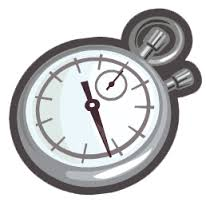
\includegraphics[width=0.75\marginparwidth]{stopwatch}
  \large\bf Opdracht \arabic{nstopdracht}}
}{%
  \end{minipage}
}

\newcounter{menucount}\newcounter{curitem}% Counters
\newcommand{\menuitem}{\texttt}% Menu item formatting
\newcommand{\menusep}{\ensuremath{\rightarrow}}% Menu separator
\newcommand{\menuend}{\relax}% Menu end
\newcommand{\menulist}[1]{% \menulist{<menu list>}
  \setcounter{menucount}{0}\setcounter{curitem}{0}% Reset menucount & curitem
  \renewcommand*{\do}[1]{\stepcounter{menucount}}%
  \menulistparser{#1}% Count menu items
  \renewcommand*{\do}[1]{\menuitem{##1}\stepcounter{curitem}\ifnumless{\value{curitem}}{\value{menucount}}{\menusep}{\menuend}}%
  \menulistparser{#1}% Process list
}
\DeclareListParser{\menulistparser}{:}% List separator is ':'


\begin{document}

\begin{center}
  \begin{mdframed}
  \centering
  \fontsize{40}{60}\selectfont Beschrijvende statistiek
  \end{mdframed}
  \vfill
  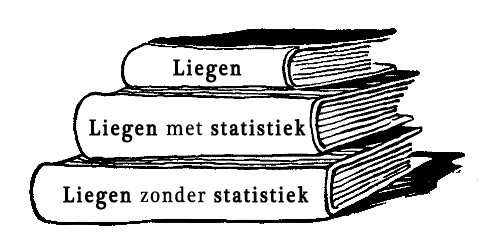
\includegraphics[width=0.8\textwidth]{statistiek_hoe_liegen}
  \vfill
\end{center}
\vfill
\subsection*{Doelstellingen}
\begin{singlespacing}
Je kan \hfill (LP 2005-069, LI 2.3.1, ET14, ET15, ET17)
\begin{itemize}
  \item het onderscheid maken tussen een steekproef en een populatie,
  \item het gemiddelde en de mediaan berekenen van statische gegevens,
  \item de interkwartielafstand en de standaardafwijking berekenen van statistische gegevens,
  \item grafische voorstellingen maken van statistische gegevens,
  \item ICT gebruiken bij de drie voorgaande doelstellingen,
  \item aan de hand van voorbeelden het belang uitleggen van de representativiteit van een steekproef voor het formuleren van statische besluiten over de populatie, hierbij functioneel gebruik maken van centrummaten, spreidingsmaten en grafische voorstellingen,
  \item kritisch omgaan met het gebruik van statistiek in de media.
\end{itemize}
\end{singlespacing}

\thispagestyle{empty}
\clearpage

\tableofcontents
\thispagestyle{empty}
\clearpage

\pagenumbering{arabic}

\pagestyle{fancy}
\fancyhead[RO,LE]{Beschrijvende statistiek}
\fancyhead[RE,LO]{}

\cleardoublepage
\section{Begrip beschrijvende statistiek}

Met beschrijvende statistiek gaan we gegevens die we bekomen door tellen, waarnemen of enquêtes kort gaan weergeven of grafisch voorstellen. Het weergeven wordt vaak gedaan met behulp van {\em kengetallen} en het grafisch voorstellen met behulp van een aantal verschillende grafieken.

Welke kengetallen we gebruiken en welke grafieken we tekenen hangt af van de bekomen gegevens en hoe volledig die gegevens zijn. De gegevens worden steeds verzameld na het stellen van een {\bf onderzoeksvraag}. Er wordt dan dezelfde enquête of meting uitgevoerd bij een aantal personen of objecten, die we de {\bf elementen} zullen noemen. Elke eigenschap die we bevragen of meten noemen een {\bf variabele}.

\begin{oefening}
Noteer bij elke onderzoeksvraag de {\bf elementen} en de {\bf variabele}:
\begin{enumerate}[(a)]
  \item Met welk vervoersmiddel komen de leerlingen naar onze school?
  \item Welke is het meest geliefde vak van alle laatstejaars leerlingen in Vlaanderen?
  \item Wat is het B.M.I. (body mass index) van de Belgen?
  \item Hoeveel computers zijn er per leerling beschikbaar voor gans Avelgem?
\end{enumerate}
\end{oefening}

\begin{oefening}
  De volgende keer dat je een M\&M snoepjes eet, denk dan eens wat er de elementen van een onderzoek zouden kunnen zijn en bedenk een tweetal variabelen die je zou kunnen onderzoeken.
\end{oefening}

\begin{oefening}
Geef zelf een onderzoeksvraag, de bijhorende elementen en variabele. Maak hier een enquête voor op.
\end{oefening}

\cleardoublepage
\section{Populatie en steekproef}

De {\bf populatie} van een statistisch onderzoek is de verzameling van alle personen of objecten die bestudeerd worden. Als we bijvoorbeeld onderzoeken met welk vervoersmiddel onze leerlingen naar school komen, dan is de populatie alle leerlingen van onze school.

Meestal is het onmogelijk of moeilijk om de hele populatie te onderzoeken. We beperken ons dan tot een deelverzameling van de hele populatie. Deze noemen we de {\bf steekproef}. Om aan alle leerlingen van onze school te vragen welk vervoersmiddel ze gebruiken zouden we te veel tijd verliezen. Daarom kunnen we er bijvoorbeeld voor kiezen om maar aan een klein deel, bijvoorbeeld elke tiende leerlingen die door de schoolpoort komt te vragen hoe ze naar school gekomen zijn.

Een steekproef moet {\bf representatief} (ze moet een juist beeld geven van de populatie, alle deelgroepen moeten namelijk evenredig vertegenwoordigd zijn), {\bf aselect} (elk element van de populatie moet dezelfde kans hebben om opgenomen te worden tot de steekproef) en {\bf groot genoeg} zijn. Deze grootte noemen we de {\bf steekproefgrootte} $n$.

\begin{oefening}
Hoe zou je ervoor kunnen zorgen dat we een goede steekproef hebben van alle leerlingen van onze school?
\end{oefening}

\begin{oefening}
Noteer van de volgende onderzoeken telkens de populatie, de steekproef en de steekproefgrootte.
\begin{enumerate}[(a)]
  \item Een interviewer vraagt telefonisch aan 500 Vlamingen of ze voor of tegen nieuwe verkiezingen zijn.
  \item Na elke rit in de Ronde van Frankrijk wordt een aantal renners onderzocht op doping.
\end{enumerate}
\end{oefening}

De eigenschap die we bestuderen noemen we de {\bf variabele}. Soms is dit een getal, bijvoorbeeld het aantal kilometer dat een leerling van school af woont, of soms niet, bijvoorbeeld het vervoermiddel dat een leerlingen gebruikt om naar school te komen. We onderscheiden soorten variabelen die dan nog onderverdeeld zijn elk in twee soorten:
\begin{itemize}
  \item {\bf Kwalitatieve variabelen}
  \begin{itemize}
    \item {\bf Nominaal}: De verschillende waarden die een variabele heeft zijn niet zinvol te vergelijken.\\
    Bijvoorbeeld: Het vervoermiddel van de leerling naar school (Te voet, Bus, Fiets, ...)
    \item {\bf Ordinaal}: De verschillende waarden die een variabele heeft kunnen geordend worden, we kunnen dus vergelijkingen maken zoals 'goed', 'beter', 'best'.\\
    Bijvoorbeeld: De tevredenheid van een televisieprogramma (*, **, ***, ****)
  \end{itemize}
  \item {\bf Kwantitatieve variabelen}
  \begin{itemize}
    \item {\bf Discreet}: De waarden zijn numeriek en bevatten onderbrekingen.\\
    Bijvoorbeeld: Het aantal gezinsleden (1, 2, 3, ...), de punten op een toets (..., 5, 5.5, 6, ...)
    \item {\bf Continue}: De waarden zijn numeriek, tussen een bepaald interval, en bevatten (minstens theoretisch) geen onderbrekingen. We kunnen dus de nauwkeurigheid zelf kiezen.\\
    Bijvoorbeeld: De afstand dat een leerling woont van school kan gegeven worden in kilometer, meter, centimeter, millimeter, ... Dus zo nauwkeurig als de onderzoeker zelf wenst.
  \end{itemize}
\end{itemize}

\begin{oefening}
Geef bij de volgende variabelen aan of het kwalitatieve of kwantitatieve variabelen zijn. Geef ook telkens één voorbeeld van een aantal mogelijke waarden.

\begin{enumerate}[(a)]
\item De smaak van fruitsnoepjes.
\item Het aantal tv-toestellen dat Vlaamse gezinnen bezitten.
\item De mate van tevredenheid bij klanten van een supermarkt.
\item De afstand die leerlingen moeten afleggen als ze naar school komen.
\end{enumerate}
\end{oefening}

\cleardoublepage
\section{Kwalitatief onderzoek}

Heel vaak krijgen we in een onderzoek een aantal verschillende waarden van een variabele die niet zinvol te vergelijken is, namelijk een nominale variabele. Zo werd er vorig jaar aan een aantal leerlingen gevraagd met welk vervoersmiddel ze naar school kwamen, volgende dataset kregen we terug:

\dataset[7]{fiets, bus, bus, auto, fiets, te voet, auto, te voet, fiets, fiets, auto, te voet, te voet, bus, bus, bus, auto, te voet, te voet, fiets, bus, bus, fiets, auto, te voet, skate board, te voet, fiets, fiets, bus, auto, bus, bus, bus, fiets, bus, te voet, te voet, fiets, auto, fiets, fiets, bus, te voet, bus, bus, fiets, bus, te voet, auto, te voet, fiets, bus, bus, bus, fiets, te voet, bus, fiets, fiets, bus}

In een {\bf dataset} is het de gewoonte om de $n$ waarneming te labelen met $x_1$, $x_2$, \ldots, $x_n$. Een aantal waarnemingen kunnen meerdere keren voorkomen, zo is $x_1=x_5=\ldots=x_{60}=$'fiets'. We maken die waarnemingen uniek door deze te labelen met $\omega_1=$'fiets' en deze krijgt dan de frequentie $n_1=17$

\subsection{Frequentietabel bij een kwalitatieve variabele}

Om vlot met deze data te kunnen werken maken we hier een {\bf frequentietabel} van, dit wil zeggen dat we de data in een tabel met op elke rij een unieke {\bf waarneming} en met de kolommen:
\begin{itemize}
  \item {\bf Waarnemingen} $\omega_j$: De unieke waarnemingen.
  \item {\bf Turven}: Manier van tellen waarbij we voor elke keer dat een waarneming voorkomt een verticaal streepje zetten, maar voor elke vijfde eenheid een groep van vier streepjes diagonaal doorhalen.
  \item {\bf Absolute frequentie} $n_j$: Aantal keren dat de waarneming voorkomt.
  \item {\bf Relatieve frequentie} $f_j$: Verhouding van de absolute frequentie van $\omega_j$ tot de steekproefgrootte $n$.\\
  Berekening: $$f_j=\dfrac{n_j}{n}$$
\end{itemize}

\begin{oefening}
Als er $k$ unieke waarnemingen $\omega_1, \omega_2, \ldots, \omega_k$ zijn, wat is dan de waarde van
$$f_1 + f_2 + \cdots f_k$$
\end{oefening}

\begin{oefening}
Maak de frequentietabel horende bij de dataset:
\dataset[7]{fiets, bus, bus, auto, fiets, te voet, auto, te voet, fiets, fiets, auto, te voet, te voet, bus, bus, bus, auto, te voet, te voet, fiets, bus, bus, fiets, auto, te voet, skate board, te voet, fiets, fiets, bus, auto, bus, bus, bus, fiets, bus, te voet, te voet, fiets, auto, fiets, fiets, bus, te voet, bus, bus, fiets, bus, te voet, auto, te voet, fiets, bus, bus, bus, fiets, te voet, bus, fiets, fiets, bus}
\end{oefening}

\begin{oefening}
In september werd aan alle leerlingen van het derde jaar gevraagd of ze een rekentoestel hadden, en zo ja, van welk merk. Vervolledig de frequentietabel.
\begin{center}
\begin{tabular}{l|c|c}
Rekenmachine & Frequentie & Rel. Freq \\\hline
Geen         &            & 0.54      \\\hline
Casio        & 27         & 0.18      \\\hline
TI           &            &           \\\hline
n=           &            &           \\
\end{tabular}
\end{center}
\end{oefening}

\begin{oefening}
 We openen een aantal zakjes {\em Gummibärchen} (kleine fruitsnoepje, gemaakt van gelatine, elk snoepje is ongeveer $2 \cm$ lang en heeft de vorm van een beertje, ze zijn beschikbaar in veel verschillende kleuren). Als we van elk beertje de kleur noteren krijgen we volgende dataset:

\dataset[10]{paars, bruin, geel, roze, blauw, oranje, paars, bruin, roze, oranje, geel, bruin, paars, bruin, bruin, geel, roze, bruin, roze, geel, blauw, oranje, paars, oranje, paars, roze, paars, oranje, bruin, geel, paars, paars, roze, geel, roze, roze, roze, roze, bruin, geel, geel, geel, paars, blauw, blauw, geel, oranje, bruin, blauw}

\begin{enumerate}[(a)]
\item Welk een soort variable hebben we?
\item Geef de frequentietabel, de relatieve frequenties mag je afronden op twee cijfers na de komma.
\item Wat zou theoretisch het antwoord zijn op $\sum_{i=1}^n f_i$.
\item In deze oefening hebben we een verschil van twee hondersten in de som van de relatieve frequenties. Waarom?
\end{enumerate}
\end{oefening}

\subsection{Grafische voorstellingen bij een kwalitatieve variabele}

\subsubsection{Staafdiagram}

Om de absolute frequentie van een kwalitatieve variabele grafisch weer te geven wordt vaak gebruik gemaakt van een staafdiagram. Op de $x$-as worden de verschillende optredende waarden van de waarnemingsgetallen gezet. Op de $y$-as wordt de overeenstemmende absolute frequentie geplaatst. Hoewel er bij een kwalitatieve variabele geen natuurlijke orde is wordt er geopteerd om steeds te ordenen van de grootste frequentie naar de kleinste frequentie. Er wordt ook afgesproken om de absolute frequentie boven elk staafje te schrijven. De staafjes mogen niet tegen elkaar staan.

Als voorbeeld zie je hier een staafdiagram
van de Vlaamse bevolking per provincie. De
informatie die hier wordt weergegeven, kan
je vinden in het boekje “Vlaanderen in
cijfers” op de website:
\url{http://www4.vlaanderen.be/dar/svr/Cijfers/Pages/Excel.aspx}.

\begin{minipage}{0.5\textwidth}
De namen van de provincies zijn afgekort als:
  \begin{description}
    \item[Antw] Antwerpen,
    \item[O-Vl] Oost-Vlaanderen,
    \item[W-Vl] West-Vlaanderen,
    \item[Vl-Br] Vlaams - Brabant,
    \item[Limb] Limburg.
  \end{description}
\end{minipage}
\begin{minipage}{0.5\textwidth}
%  \definecolor{qqqqff}{rgb}{0,0,1}
\begin{tikzpicture}[scale=0.1,line cap=round,line join=round,>=triangle 45,x=1.0cm,y=1.0cm]
\draw[-,color=black] (-9.63,0) -- (78.66,0);
\draw[color=black] (60,0.13) node [anchor=south west] { Provincie};
\draw[-,color=black] (0,-4.46) -- (0,27.9);
\draw[color=black] (0.57,27.25) node [anchor=west] { Aantal inwoners};
\clip(-9.63,-4.46) rectangle (78.66,27.9);
\draw[fill=black,fill opacity=0.1] (7,0) rectangle (12.5,8.39);
\draw[fill=black,fill opacity=0.1] (12.5,0) rectangle (17.5,0);
\draw[fill=black,fill opacity=0.1] (17.5,0) rectangle (22.5,10.77);
\draw[fill=black,fill opacity=0.1] (22.5,0) rectangle (27.5,0);
\draw[fill=black,fill opacity=0.1] (27.5,0) rectangle (32.5,11.59);
\draw[fill=black,fill opacity=0.1] (32.5,0) rectangle (37.5,0);
\draw[fill=black,fill opacity=0.1] (37.5,0) rectangle (42.5,14.32);
\draw[fill=black,fill opacity=0.1] (42.5,0) rectangle (47.5,0);
\draw[fill=black,fill opacity=0.1] (47.5,0) rectangle (52.5,17.45);
\draw (48.1,-0.39) node[anchor=north west] {Antw};
\draw (18.33,-0.43) node[anchor=north west] {Vl-Br};
\draw (28.4,-0.43) node[anchor=north west] {W-Vl};
\draw (38.13,-0.43) node[anchor=north west] {O-Vl};
\draw (7.91,-0.36) node[anchor=north west] {Limb};
\draw (46.85,24) node[anchor=north west] {1744862};
\draw (16.74,18) node[anchor=north west] {1076924};
\draw (26.93,12.35) node[anchor=north west] {1159366};
\draw (36.66,15.08) node[anchor=north west] {1432326};
\draw (7.23,9.13) node[anchor=north west] {838505};
\begin{scriptsize}
\fill [color=qqqqff] (0,0) circle (1.5pt);
\end{scriptsize}
\end{tikzpicture}

  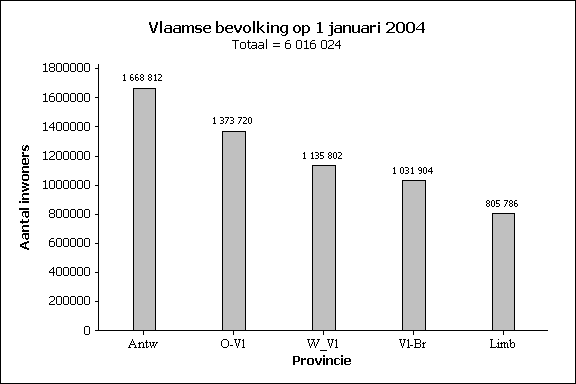
\includegraphics[width=8cm]{vlaamse_bevolking.png}
\end{minipage}

\begin{oefening}
Gebruik de frequentietabel:
\begin{center}
  \begin{tabular}{c|c|c}
    $\omega_i$ & $n_i$ & $f_i$\\
    \hline
    fiets      & 17    & 0.28\\
    bus        & 21    & 0.34\\
    auto       &  8    & 0.13\\
    te voet    & 14    & 0.23\\
    skate board&  1    & 0.02
  \end{tabular}
\end{center}
Om een staafdiagram te maken.
\end{oefening}

\begin{oefening}
  Aan 24 studenten werd gevraagd om een even getal tussen 0 en 9 te noemen en daarbij werd de volgende reeks getallen geregistreerd:

  \begin{center}
    \dataset[10]{2, 6, 4, 0, 6, 8, 6, 4, 2, 4, 0, 6, 8, 0, 0, 2, 4, 6, 8, 4, 0, 2, 2, 0,}
  \end{center}
  \begin{enumerate}[(a)]
  \item Maak de frequentietabel.
  \item Teken het staafdiagram.
\end{enumerate}
\end{oefening}

\subsubsection{Schijfdiagram}

\begin{minipage}{0.5\linewidth}
Een {\bf schijfdiagram} of {\bf taartdiagram} is een grafische voorstelling van de relatieve frequenties.Bij het tekenen van een taartdiagram verdeel je een cirkeloppervlak in stukken, juist zoals je een taart in stukken snijdt. Eén zo'n stuk heet een {\bf sector}. De totale oppervlakte van de cirkel komt overeen met de som van alle percentages en dat is 100\%.

Voor een taartdiagram maken we enkele afspraken:
\begin{itemize}
  \item Begin bovenaan en draai met de wijzers van de klok mee.
  \item De grootste sector komt eerst, dan komt de tweede
grootste, enzovoort.
\end{itemize}

Je ziet hier een voorbeeld van de marktaandelen van energiebevoorraders in België. Het gaat over de elektriciteit in het jaar 2004. Deze figuur staat in het weekblad Knack van 22 juni 2005 en is goed leesbaar. Maar als je een krant of weekblad doorbladert, dan zie je soms verwarrende en zelfs verkeerde grafieken.
\end{minipage}
\begin{minipage}{0.5\linewidth}
\begin{center}
  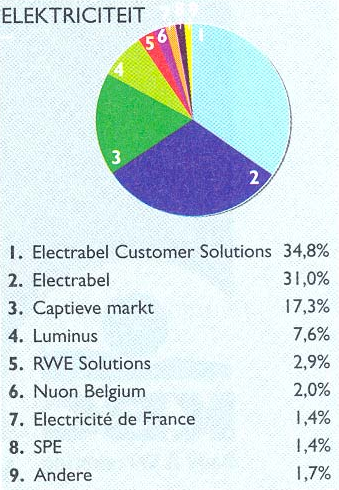
\includegraphics[width=0.9\textwidth]{cirkeldiagram_electriciteit}
\end{center}
\end{minipage}

Hoeveel graden elke sector is, bereken je door de relatieve frequentie te vermenigvuldigen met $360\degree$. Dit doe je met je rekenmachine. Maak daarna “verstandige” afrondingen zodat alle sectoren samen terug $360\degree$ geven (je kan eventueel enkele keren tot op een halve graad werken).

\begin{oefening}
Gebruik de frequentietabel:
\begin{center}
  \begin{tabular}{c|c|c}
    $\omega_i$ & $n_i$ & $f_i$\\
    \hline
    fiets      & 17    & 0.28\\
    bus        & 21    & 0.34\\
    auto       &  8    & 0.13\\
    te voet    & 14    & 0.23\\
    skate board&  1    & 0.02\\
  \end{tabular}
\end{center}
Om een cirkeldiagram te maken.\\
{\em Hint: Voeg eerst een kolom toe waarin je de hoek van elke sector berekend.}
\end{oefening}

\begin{oefening}
We vragen aan een aantal mensen wat hun lievelingskleur is en krijgen volgende antwoorden:
\dataset[6]{rood, paars, groen, rood, groen, geel, purper, oranje, hemelsblauw, groen, rood, paars, geel, geel, zwart, groen, lichtgroen, oranje, geel, rood, oranje, groen, geel, groen, geel, blauw, rood, groen, oranje, blauw, rood, geel, groen, rood, paars, groen, rood, rood, blauw, geel, rood}
\begin{enumerate}[(a)]
\item Terwijl je turft kan je de dataset eigenlijk vereenvoudigen. Welke aannames kan je hier maken?
\item Maak een taartdiagram.
\end{enumerate}
\end{oefening}


\begin{oefening}
Ik vraag aan een aantal leerlingen welk vak ze graag doen. De leerlingen antwoorden heel ''eerlijk''. Ik turf de dataset en krijg volgende frequentietabel:

\begin{center}
  \begin{tabular}{r|ccccc}
    Vak  & Wiskunde & Natuurwetenschappen & Nederlands & Frans & Duits \\
    \hline
    Freq & 12       & 3                   & 8          & 4     & 6     \\
  \end{tabular}
\end{center}

\begin{enumerate}[(a)]
\item Wat is hier de variabele en welk soort variabele is het?
\item Maak de frequentietabel opnieuw, maar nu zodanig dat er kolommen met berekeningen toegevoegd kunnen worden.
\item Welk een figuur past er hier best bij de relatieve frequentie?
\item Welk een kolom moet je toevoegen?
\item Maak deze figuur.
\end{enumerate}
\end{oefening}

\pagebreak
\subsection{Kwalitatief onderzoek in de media}

\begin{oefening}

Soms kom je de uitdrukking “horizontaal staafdiagram” tegen. Kijk daarvoor naar de figuur die je vindt in de Gazet van Antwerpen van 3 november 2004. Voor de 364 jobs die in oktober 2004 bij de 4 grootste faillissementen in Vlaanderen verloren gingen, heeft men een figuur getekend.

\begin{center}
  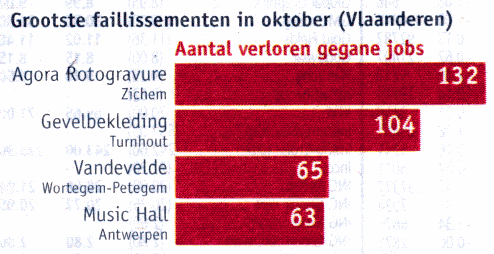
\includegraphics[width=0.5\textwidth]{horizontaal_staafdiagram-faillissementen}
\end{center}

\begin{enumerate}[(a)]
\item Welke variabele is er genoteerd bij elke persoon die zijn job is kwijtgeraakt?
\item Welk soort variabele is dat?
\item Wat zijn haar waarden?
\item Is de figuur goed getekend?
\end{enumerate}
\end{oefening}

\begin{oefening}
Als je een frequentietabel ziet, dan moet je die juist kunnen interpreteren. Bekijk de tabel over XTC en Speed (Gazet van Antwerpen van 20-10-2004). Kijk enkel naar de informatie die daarin staat over het jaar 2003.

\begin{center}
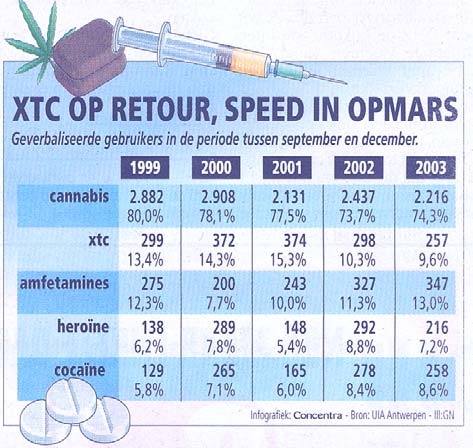
\includegraphics[width=0.6\textwidth]{tabel-drugs}
\end{center}

\begin{enumerate}[(a)]
  \item Is “druggebruik” daar behandeld als een kwalitatieve variabele?
  \item Is de tabel correct?
\end{enumerate}
\end{oefening}

\begin{oefening}
Een bestaande figuur moet je juist kunnen interpreteren. Bekijk het taartdiagram over de
vrijetijdsbesteding van jongeren (De Standaard van 6-12-2000).

\begin{center}
  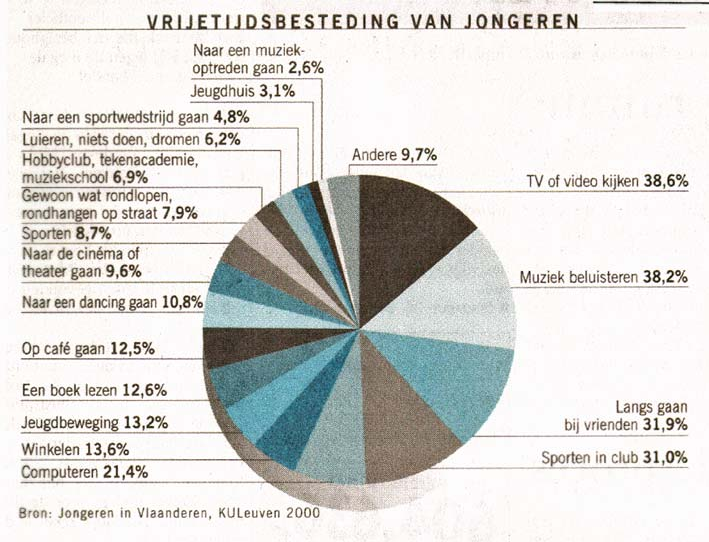
\includegraphics[width=1\textwidth]{cirkeldiagram-vrijetijdsbesteding}
\end{center}

\begin{enumerate}[(a)]
  \item Is “vrijetijdsbesteding” hier behandeld als een kwalitatieve variabele?
  \item Is het taartdiagram correct getekend?
\end{enumerate}
\end{oefening}

\cleardoublepage
\section{Kwantitatief onderzoek}

We herinneren ons dat we met een kwantitatieve variabele kunnen rekenen. We beschouwen nu een voorbeeld waarbij de directeur een aantal jaar terug de tijd heeft opgemeten dat het duurt voordat de leerling aan de les beginnen nadat het belsignaal heeft gerinkeld. We krijgen een lijst van 65 getallen waarbij elk getal een tijdstip in seconden voorstelt:

\dataset[10]{193, 225, 256, 166, 143, 260, 117, 208, 182, 114, 113, 203, 320, 231, 221, 231, 60, 113, 373, 180, 379, 205, 161, 287, 196, 236, 163, 192, 184, 166, 332, 172, 227, 272, 264, 155, 296, 189, 119, 230, 253, 225, 194, 200, 91, 177, 208, 157, 243, 183, 89, 235, 190, 223, 186, 132, 235, 312, 125, 258, 98, 173, 165, 289, 262}

\subsection{Een frequentietabel met klassenindeling}

Je beschikt nu over een groot aantal opmetingen van een continu kwantitatieve variabele. In feite is elke geschatte tijdsduur verschillend van elke andere, maar daarvoor had je moeten meten tot op een miljardste van een seconde (of misschien nog preciezer!). Als elke “echte” waarde verschillend is van elke andere, dan komt elke “echte” waarde slechts één keer voor. Een frequentietabel zou dan (theoretisch) al die verschillende “echte” waarden moeten bevatten, allemaal met een frequentie gelijk aan één. Dat is zinloos.

De tijdsmetingen die je hier hebt, worden, zoals alle continue variabelen, samengevat in een
{\bf frequentietabel met klassenindeling}.

\begin{center}
  \begin{tabular}{|c|c|}
    \hline
    Klasse & Frequentie\\
    \hline
    $[60;65[$ & $1$\\
    \hline
    $[65;70[$ & $0$\\
    \hline
    $[70;75[$ & \ldots\\
    \hline
    \ldots & \ldots\\
    \hline
  \end{tabular}
\end{center}

Voor het maken van de klassen kan je als volgt te werk gaan.
\begin{itemize}
  \item Start met een interval dat groot genoeg is om al je opmetingen te kunnen bevatten. Als je kleinste observatie 60 is en je grootste is 379, dan moet je dus minstens van 60 tot 379 gaan. Meestal neem je eenvoudige “ronde” getallen. Hier zou je bijvoorbeeld kunnen starten bij 60 en eindigen bij 380 of 390 (13 keer een halve minuut).
  \item Op dit grote interval maak je nu deelintervallen die mooi aan elkaar aansluiten en elkaar niet overlappen. Dat zijn je klassen. De breedte van die klassen mag je zelf kiezen en ze hoeven zelfs niet allemaal even breed te zijn.
  \item Elke klasse is een “links gesloten – rechts open” interval, zoals bijvoorbeeld $[60;65[$. De grenzen van een klasse heten {\bf klassengrenzen}. Het midden heet {\bf klassenmidden} en de breedte heet {\bf klassenbreedte}.
  \item Zorg ervoor dat het overgrote deel van de waarnemingen niet binnen één of twee klassen valt. Als richtlijn neem je tussen de 5 en de 15 klassen, maar deze richtlijn hoef je niet te strikt te nemen. Als je de frequentietabel gebruikt om een histogram te tekenen (zoals uitgelegd in volgend puntje), dan zal je ervaren dat te veel klassen dikwijls een zeer onrustige figuur geven terwijl te weinig klassen bijna niets meer tonen.
\end{itemize}

\begin{minipage}{0.8\linewidth}
Als de tabel gemaakt is, dan kan het turven beginnen. {\bf Turven} is tellen door streepjes per vijf te groeperen. Dit doe je door de elementen van je dataset te overlopen en voor elk element een streepje te plaatsen bij de correcte klasse.
\end{minipage}
\begin{minipage}{0.2\linewidth}
\begin{center}
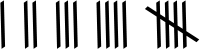
\includegraphics[width=0.9\textwidth]{turven}
\end{center}
\end{minipage}

Naast de frequentie en de relatieve frequentie bestaan er ook nog de {\it cumulatieve} versies van deze frequenties. Cumulatief wil zeggen dat iets steeds toeneemt of ophoopt. In het geval van de frequentie is de {\bf cumulatieve frequentie} het aantal gegevens dat tot deze klasse en alle lagere klassen behoord. De {\bf relatieve cumulatieve frequentie} van een klasse is dan de verhouding van de cumulatieve frequentie van die klasse en het totale aantal gegevens.

\begin{oefening}
  Stel nu een frequentietabel voor de volgende dataset. Kies een verstandige klassenbreedte.
  \dataset[10]{
193, 225, 256, 166, 143, 260, 117, 208, 182, 114, 113, 203, 320, 231, 221, 231, 60, 113, 373, 180, 379, 205, 161, 287, 196, 236, 163, 192, 184, 166, 332, 172, 227, 272, 264, 155, 296, 189, 119, 230, 253, 225, 194, 200, 91, 177, 208, 157, 243, 183, 89, 235, 190, 223, 186, 132, 235, 312, 125, 258, 98, 173, 165, 289, 262
}
\end{oefening}

\begin{oefening}
  Gemiddeld is een basketbal speler $2.01 \m$ groot. Op de website van de (National Basketball Association) NBA vinden we volgende dataset.
  \dataset[10]{
    1.93, 2.22, 2.08, 2.26, 1.98, 2.13, 2.16, 1.94, 1.89, 1.96, 1.92, 2.09, 2.11, 2.09, 2.13, 2, 1.67, 2.08, 2.2, 2.18, 2.18, 2.17, 1.96, 1.95, 2.01, 2.07, 1.74, 1.81, 2.04, 1.99, 1.99, 1.91, 1.74, 2.12, 1.95, 2, 2.25, 2.29, 1.9, 1.98, 2.03, 2.16, 1.82, 2.17, 1.92, 1.99, 1.95, 2, 2, 1.91, 2.26, 2.21, 2.31, 1.91, 2.1, 2.09, 2.17, 1.98, 1.95, 1.96, 2.21, 2.18, 1.96, 1.82, 1.89, 2.21, 2.09, 1.87, 1.83, 2.16, 1.87, 2.18, 2.09, 2.1, 1.7, 2.01, 2.2, 1.67, 1.87, 2.14
  }
  Maak een goede frequentietabel.
\end{oefening}

\begin{oefening}
  In een klas met 24 leerlingen geef ik een onverwachte toets op 10. Volgende resultaten werden behaald en op score geplaatst:
  \begin{center}
    \dataset[10]{
      7.5, 9, 9, 5.5, 8.5, 7.5, 7, 9, 7.5, 3, 8.5, 6, 8, 8.5, 7.5, 8, 9, 7, 9, 7, 7, 8, 6, 8
    }
  \end{center}
  Is het hier nodig om een frequentietabel te maken met klassen?
\end{oefening}

\subsection{Het histogram}

Een {\bf histogram} is de meest gebruikte figuur om het globale gedrag van continu
kwantitatieve gegevens te onderzoeken. Deze stelt de frequentieverdeling bij klassenindeling
grafisch voor. We maken een histogram als volgt:

\begin{enumerate}
  \item Kies op de $x$-as een lengte-eenheid en breng op de $x$-as de beeldpunten van de klassengrenzen aan. Elke klasse komt dan overeen met een lijnstuk.
  \item De klassenfrequenties worden voorgesteld met behulp van rechthoeken die de horizontale lijnstukken op de $x$ as als zijde hebben. Dan moet de verticale zijde zo zijn, dat de oppervlakte van de bijbehorende rechthoek recht evenredig is met de frequentie van een klasse. We moeten dus de hoogte van elke rechthoek berekenen en vervolgens die rechthoeken construeren, allen aan de zelfde kant van de $x$-as.
\end{enumerate}

Vaak zal men boven het histogram ook nog een {\bf frequentiepolygoon} tekenen. Hierbij verbind men het hoogste punt van de staafjes binnen het histogram in het klassenmidden met elkaar. Soms wordt voor de kleinste waarde en na de grootste waarde nog twee fictieve waarden toevoegen, elk met frequentie nul, zodat de frequentiepolygoon begint en eindigt op de $x$-as.

\subsubsection*{Verschil tussen een staafdiagram en een histogram}
Sommigen denken dat een histogram en een staafdiagram goed op elkaar lijken. Dat is fout, want er zijn fundamentele verschillen. Een histogram hoort bij een continu kwantitatieve variabele waar geen tussenstappen zijn tussen de “mogelijke” uitkomsten. Bij een histogram liggen de rechthoeken dus tegen elkaar. Bij een staafdiagram is er open ruimte tussen de staafjes. Bovendien kijk je bij een staafdiagram naar de hoogte en bij een histogram naar de oppervlakte.

\begin{oefening}
Teken het histogram en het frequentiepolygoon horende bij volgende frequentietabel.\\
\begin{center}
\begin{tabular}{c|c|c|c}
$i$ & klasse     & $n_i$ & $f_i$\\
\hline
  1 & $[ 60,  90[$ &   2 &  0.03\\
  2 & $[ 90, 120[$ &   7 &  0.11\\
  3 & $[120, 150[$ &   3 &  0.05\\
  4 & $[150, 180[$ &  10 &  0.15\\
  5 & $[180, 210[$ &  16 &  0.25\\
  6 & $[210, 240[$ &  11 &  0.17\\
  7 & $[240, 270[$ &   7 &  0.11\\
  8 & $[270, 300[$ &   4 &  0.06\\
  9 & $[300, 330[$ &   2 &  0.03\\
 10 & $[330, 360[$ &   1 &  0.02\\
 11 & $[360, 390[$ &   2 &  0.03\\
\end{tabular}
\end{center}
\end{oefening}

\begin{oefening}
In een klas met 24 leerlingen geef ik een onverwachte toets op 10. Volgende resultaten werden behaald en op score geplaatst:
\begin{center}
\dataset[10] {
  7.5, 9, 9, 5.5, 8.5, 7.5, 7, 9, 7.5, 3, 8.5, 6, 8, 8.5, 7.5, 8, 9, 7, 9, 7, 7, 8, 6, 8
}
\end{center}
\begin{enumerate}[(a)]
\item Je kan hier kiezen om de dataset onder te verdelen in klassen, waarbij de klassen geen interval zijn, maar de waarnemingen zelf.
\item Maak dan een staafdiagram.
\item Maak dan een histogram.
\end{enumerate}
\end{oefening}


\begin{oefening}
Als je de groottes van de basketbalspelers in acht klassen hebt opgedeeld krijgen we volgende frequentietabel. Maak zelf het bijhorende histogram en teken het frequentiepolygoon.\\
\begin{center}
\begin{tabular}{c|c|c}
$i$ & klasse     & $n_i$\\
\hline
  1 & $[ 1.60,  1.70[$ &   2\\
  2 & $[ 1.70,  1.80[$ &   3\\
  3 & $[ 1.80,  1.90[$ &   9\\
  4 & $[ 1.90,  2.00[$ &   22\\
  5 & $[ 2.00,  2.10[$ &   16\\
  6 & $[ 2.10,  2.20[$ &   17\\
  7 & $[ 2.20,  2.30[$ &   10\\
  8 & $[ 2.30,  2.40[$ &   1\\
\end{tabular}
\end{center}
\end{oefening}

\subsection{Numerieke kenmerken: de kengetallen}

Jij en je buur kunnen elkaars punten van het rapport vergelijken. Elke reeks punten van een rapport kan je zien als een reeks waarnemingsgetallen. Hiervan zou je bijvoorbeeld elkaars gemiddelde kunnen vergelijken of hoe de punten verspreid liggen.

Je zou ook een onderzoek kunnen doen naar lichaamsgrootte binnen een aantal verschillende sporten. Je kan bijvoorbeeld 100 basketters interviewen en 150 volleybalspelers. Van de bekomen reeksen van klassen kunnen we ook weer bepaalde {\bf kengetallen} berekenen. We zullen onderscheid maken tussen centrummaten en spreidingsmaten.

\subsubsection{Centrummaten}

{\bf Centrummaten} geven de waarde waar rond de waarnemingsgetallen gecentreerd zijn. Ze tonen ons het midden van de data.

De ons best gekende is het {\bf gemiddelde} $\bar{x}$. Bij een reeks van $n$ waarnemingsgetallen $x_1$, $x_2$, $\ldots$, $x_n$ berekenen we het gemiddelde met
$$\bar{x}=\dfrac{x_1 + x_2 + \cdots + x_n}{n}$$
We kunnen dit korter schrijven als
$$\bar{x}=\dfrac{1}{n}\sum^n_{i=1}x_i$$
Als we een indeling in klassen hebben kunnen we niet langer het gemiddelde exact bepalen. We berekenen dan een schatting als volgt:
\begin{enumerate}
  \item Bereken van alle klassen het klassenmidden.
  \item Bereken het product van het klassenmidden met de frequentie.
  \item Bepaal de som van de voorgaande producten.
  \item Deel deze som door de steekproefgrootte $n$.
\end{enumerate}

\begin{oefening}
Bepaal het gemiddelde van de volgende toetsresultaten:
\begin{center}
\dataset[10]{7.5, 9, 9, 5.5, 8.5, 7.5, 7, 9, 7.5, 3, 8.5, 6, 8, 8.5, 7.5, 8, 9, 7, 9, 7, 7, 8, 6, 8}
\end{center}
\end{oefening}

\begin{oefening}
Bepaal het gemiddelde van de volgende frequentietabel
\begin{center}
\begin{tabular}{c|c|c}
$i$ & klasse     & $n_i$\\
\hline
  1 & $[ 1.60,  1.70[$ &   2\\
  2 & $[ 1.70,  1.80[$ &   3\\
  3 & $[ 1.80,  1.90[$ &   9\\
  4 & $[ 1.90,  2.00[$ &   22\\
  5 & $[ 2.00,  2.10[$ &   16\\
  6 & $[ 2.10,  2.20[$ &   17\\
  7 & $[ 2.20,  2.30[$ &   10\\
  8 & $[ 2.30,  2.40[$ &   1\\
\end{tabular}
\end{center}
\end{oefening}

De volgende centrummaat is de {\bf mediaan} Med, dit is het getal zodat er evenveel getallen kleiner dan of gelijk zijn aan de mediaan als dat er getallen groter dan of gelijk zijn aan de mediaan. Bij een reeks waarnemingsgetallen berekenen we de mediaan als volgt $x_1$, $x_2$, $\ldots$, $x_n$:
\begin{itemize}
  \item $n$ is oneven: We nemen het middelste getal na het ordenen van de getallen.
  \item $n$ is even: We nemen het gemiddelde van de twee middelste getallen na het ordenen van de getallen.
\end{itemize}
Als we een indeling in klassen hebben nemen we het klassenmidden (of het gemiddelde van de klassenmiddens bij een even steekproefgrootte) van de klasse waar de middelste waarneming zich bevind. Merk op dat het interessant is om hiervoor de kolom met cumulatieve frequenties te gebruiken.

\begin{oefening}
Bepaal de mediaan van de volgende toetsresultaten:
\begin{enumerate}[(a)]
  \item \dataset[10]{5, 4, 4, 7, 7}
  \item \dataset[10]{5, 7.5, 4, 8, 6, 8}
  \item \dataset[10]{6, 7, 6, 6, 6, 7, 6, 10}
\end{enumerate}
\end{oefening}

\begin{oefening}
Bepaal de mediaan van de volgende frequentietabelen
\begin{multicols}{2}
\begin{enumerate}[(a)]
  \item
  \begin{center}
\begin{tabular}{c|c|c}
$i$ & klasse     & $n_i$\\
\hline
  1 & $[ 1.60,  1.70[$ &   2\\
  2 & $[ 1.70,  1.80[$ &   3\\
  3 & $[ 1.80,  1.90[$ &   9\\
  4 & $[ 1.90,  2.00[$ &   22\\
  5 & $[ 2.00,  2.10[$ &   16\\
  6 & $[ 2.10,  2.20[$ &   17\\
  7 & $[ 2.20,  2.30[$ &   10\\
  8 & $[ 2.30,  2.40[$ &   1\\
\end{tabular}
\end{center}
  \item
  \begin{center}
\begin{tabular}{c|c|c}
$i$ & klasse     & $n_i$\\
\hline
  1 & $[ 1.60,  1.70[$ &   2\\
  2 & $[ 1.70,  1.80[$ &   3\\
  3 & $[ 1.80,  1.90[$ &   9\\
  4 & $[ 1.90,  2.00[$ &   22\\
  5 & $[ 2.00,  2.10[$ &   17\\
  6 & $[ 2.10,  2.20[$ &   17\\
  7 & $[ 2.20,  2.30[$ &   10\\
  8 & $[ 2.30,  2.40[$ &   1\\
\end{tabular}
\end{center}
\end{enumerate}
\end{multicols}
\end{oefening}

Tot slot is er nog de {\bf modus} Mod. Bij een reeks waarnemingsgetallen $x_1$, $x_2$, $\ldots$, $x_n$ is dat de waarneming die het meeste voorkomt. Als er meerdere waarneming de hoogste frequentie hebben is de modus een verzameling van deze waarnemingsgetallen. Bij een indeling in klassen nemen we de klassen met de hoogste frequentie als als modus, we noemen deze dan de {\bf modale klasse}.

We merken verder op dat het gemiddelde veel gevoeliger is dan de mediaan. Wat we hiermee bedoelen is dat, indien er in een reeks waarnemen extreme waarden voorkomen die eigenlijk onmogelijk zouden zijn, dat het gemiddelde hierdoor beïnvloed wordt. De mediaan kan dus soms een betere centrummaat zijn.

\begin{oefening}
In een fabriek worden 1 liter flessen gevuld met ketchup. Om te controleren dat er geen fout zit op de machine wordt er elk uur steekproefgewijs 8 flessen gewogen. We krijgen volgende data de maandagmorgen:
\dataset[8]{230 gr, 1202 gr, 1212 gr, 1183 gr, 1191 gr, 1236 gr, 1232 gr, 1193 gr}
\begin{enumerate}[(a)]
  \item Bepaal het gemiddelde.
  \item Bepaal de mediaan.
  \item Welk centrum past hier het best bij de data en waarom?
\end{enumerate}
\end{oefening}

\subsubsection{Spreidingsmaten}

Met {\bf spreidingsmaten} kunnen we met getallen weergeven hoe de waarnemingsgetallen verspreid liggen rond een centrummaat. Beschouw bijvoorbeeld volgende twee datasets
\begin{center}
  \texttt{4\; 6\; 8\; 10} \qquad\qquad en \qquad\qquad \texttt{1\; 4\; 5\; 9\; 11\; 12}
\end{center}
Beide reeksen hebben hetzelfde gemiddelde en dezelfde mediaan. Toch is er een verschil, namelijk de linker dataset ligt dichter ronde het gemiddelde en de mediaan dan de rechter dataset. We zeggen dat de spreiding links kleiner is.

De eenvoudigste spreidingsmaat is de {\bf variatiebreedte} $R$. Deze geeft ons de afstand tussen het kleinste en grootste getal van een reeks waarnemingen $x_1$, $x_2$, $\ldots$, $x_n$:
$$R=\max_{i=1}^n x_i - \min_{i=1}^n x_i $$
Bij een indeling in klassen wordt de afstand tussen de kleinste en grootste klassenmidden berekend.

\begin{oefening}
Bepaal de variatiebreedte van volgende waarnemingsgetallen:
\begin{center}
\dataset[10]{7.5, 9, 9, 5.5, 8.5, 7.5, 7, 9, 7.5, 3, 8.5, 6, 8, 8.5, 7.5, 8, 9, 7, 9, 7, 7, 8, 6, 8}
\end{center}
\end{oefening}

\begin{oefening}
Bepaal de variatiebreedte van de volgende frequentietabel
\begin{center}
\begin{tabular}{c|c|c}
$i$ & klasse     & $n_i$\\
\hline
  1 & $[ 1.60,  1.70[$ &   2\\
  2 & $[ 1.70,  1.80[$ &   3\\
  3 & $[ 1.80,  1.90[$ &   9\\
  4 & $[ 1.90,  2.00[$ &   22\\
  5 & $[ 2.00,  2.10[$ &   16\\
  6 & $[ 2.10,  2.20[$ &   17\\
  7 & $[ 2.20,  2.30[$ &   10\\
  8 & $[ 2.30,  2.40[$ &   1\\
\end{tabular}
\end{center}
\end{oefening}

Een weinig gebruikte spreidingsmaat is de {\bf gemiddelde absolute afwijking} $Mad$ die de gemiddelde afstand van een reeks waarnemingsgetallen $x_1$, $x_2$, $\ldots$, $x_n$ bepaalt:
$$Mad=\dfrac{1}{n}\sum_{i=1}^n|x_i-\bar{x}|$$

Wij laten deze buiten beschouwing daar deze in de praktijk toch niet gebruikt wordt. Wel vaak gebruikt zijn de {\bf variatie} $s^2$ die het gemiddelde van het kwadraat van de afstanden van een reeks waarnemingen $x_1$, $x_2$, $\ldots$, $x_n$ bepaalt:
$$s^2=\dfrac{1}{n}\sum_{i=1}^n(x_i-\bar{x})^2$$
Door het kwadraat krijgen we echter een vertekeningen, daarom werd de {\bf standaardafwijking} $s$ ingevoerd:
$$s=\sqrt{\dfrac{1}{n}\sum_{i=1}^n(x_i-\bar{x})^2}$$

Om bij een indeling in klassen de variatie en standaardafwijking te berekenen gebruiken we opnieuw de producten die bekomen worden door het klassenmidden te vermenigvuldigen met de frequentie. We verkiezen echter om deze kengetallen te berekenen met het \zrm{ZRM}.

Een andere maat voor spreiding is de lengte van het gebied waarin de middelste 50\% van de
geordende opmetingen liggen. Dit gebied loopt van het {\bf eerste kwartiel} $Q_1$ tot het {\bf derde kwartiel} $Q_3$.
De lengte van dit interval is de {\bf interkwartielafstand}, genoteerd als $IQR$ (= InterQuartile Range).
Als we de reeds berekende mediaan $Q_2$ noemen, dan is $Q_1$ te bepalen door de mediaan te nemen van de
gegevens links van $Q_2$ en $Q_3$ is te bepalen door de mediaan te nemen van de gegevens rechts van $Q_2$. Ook
dit kengetal zullen we berekenen met software.

\subsubsection{Berekenen van de 1-variabele statistieken}

Alle voorgaande kengetallen vatten we samen met de {\bf 1-variabele statistieken}. Deze kunnen allemaal
in één keer berekend worden met het \zrm{ZRM}. De instructies zijn afhankelijk van het rekentoestel. Ook geeft het nieuwe rekentoestel iets meer kengetallen. Het verschil is echter niet groot, een nieuwer rekentoestel heb je zeker niet nodig voor de oefeningen.

\begin{minipage}{\textwidth}
\begin{multicols}{2}

\begin{center}
  \begin{mdframed}Nieuw model: fx-92B Spéciale Collège\end{mdframed}
\end{center}\mbox{}\\
Kies \zrm{MENU} en daarna \zrm{2:Statistics} en \zrm{EXE}. Nu kan de juiste soort statistische variabele, \zrm{1:1-Variable} gekozen worden waarna alle waarnemingen ingevoerd kunnen worden. Kies daarna het \zrm{OPTN} en \zrm{3:1-Variable Calc}.

\vfill\columnbreak

\begin{center}
  \begin{mdframed}Oud model: fx-92B Collège 2D+\end{mdframed}
\end{center}\mbox{}\\
Kies \zrm{MODE} en daarna \zrm{2:STAT} en \zrm{EXE}. Nu kan de juiste soort statistische variabele, \zrm{1:1-VAR} gekozen worden waarna alle waarnemingen ingevoerd kunnen worden. Druk daarna op \zrm{AC}. Nu ben je in rekengedeelte van de statistiek mode. De \verb#0# die daar staat is normaal. Nu kan je de verschillende statistieken uitrekenen met \zrm{SHIFT} \zrm{STAT} (bij het knopje van 1). Kies daar \zrm{4:Var} en dan \zrm{2:$\bar{x}$} voor gemiddelde of \zrm{3:s$x$} voor de standaard afwijking.

\end{multicols}
\end{minipage}

De volgende zijn belangrijk:
\begin{center}
  \begin{tabular}{r|l}
    $\bar{x}$ & Het gemiddelde.\\
    $s^2x$ & De variatie.\\
    $sx$ & De standaard afwijking.\\
    $n$ & De steekproefgrootte.\\
    $min(x)$ & De laagste waarde.\\
    $Q_1$ & Het eerste kwartiel.\\
    $Med$ & De mediaan.\\
    $Q_3$ & Het derde kwartiel.\\
    $max(x)$ & De hoogste waarde.\\
  \end{tabular}
\end{center}

\begin{oefening}
Bepaal de 1-variabele statistieken van volgende waarnemingsgetallen m.b.v. het \zrm{ZRM}:
\begin{center}
\dataset[10]{7.5, 9, 9, 5.5, 8.5, 7.5, 7, 9, 7.5, 3, 8.5, 6, 8, 8.5, 7.5, 8, 9, 7, 9, 7, 7, 8, 6, 8}
\end{center}
\end{oefening}

\begin{oefening}
Door 88 willekeurige 17 jarigen wordt een IQ test afgelegd. De dataset krijgen we niet, maar we krijgen wel volgende frequentietabel met klassenindeling:
\begin{center}
  \begin{tabular}{c|c}
    Interval & Frequentie\\
    \hline
    $[50, 60[$ & 2\\
    $[60, 70[$ & 2\\
    $[70, 80[$ & 5\\
    $[80, 90[$ & 25\\
    $[90, 100[$ & 22\\
    $[100, 110[$ & 16\\
    $[110, 120[$ & 11\\
    $[120, 130[$ & 5
  \end{tabular}
\end{center}

\begin{enumerate}[(a)]
  \item Teken het histogram, gebruik een blauwe balpen.
  \item Teken op het histogram het frequentiepolygoon, gebruik een groene balpen.
  \item Wat is het gemiddelde?
  \item Wat is de mediaan?
  \item Wat de modus?
\end{enumerate}
\end{oefening}

\needspace{8cm}
\subsection{De boxplot}

\begin{wrapfigure}[9]{l}{0.4\textwidth}
  \vspace{-1cm}
  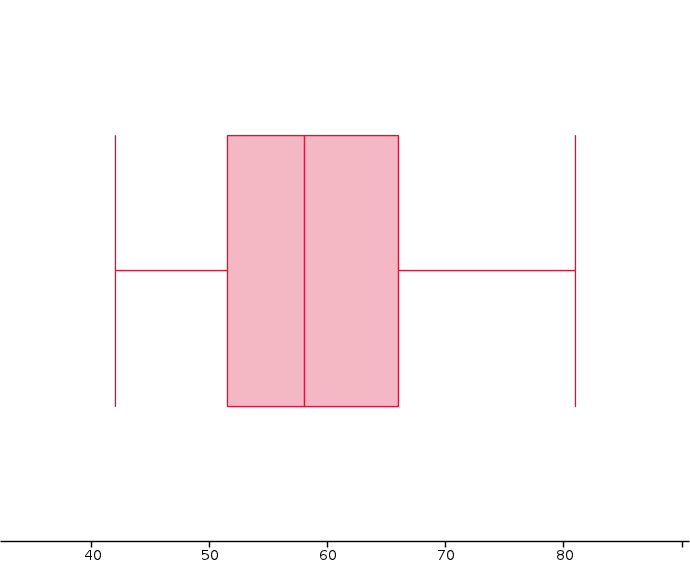
\includegraphics[width=0.4\textwidth]{boxplot}
\end{wrapfigure}

Een goed zicht op zowel het centrum als de spreiding van je opmetingen, krijg je uit een boxplot. Dit
is een grafiek die gebruik maakt van de begrippen minimum, maximum, mediaan, eerste kwartiel
Q1, derde kwartiel Q3, IQR en uitschieters.

De rechterstaart begint vanaf Q3. Dit lijnstuk gaat tot aan de grootste opmeting die kleiner of
gelijk is aan $\mbox{Q3} + (1.5\cdot\mbox{IQR})$. Elke observatie die nog groter is, wordt als een uitschieter
beschouwd en apart aangeduid. In deze studie loopt de rechterstaart van $66$ tot $81$ en heeft
dus een lengte van $15$. Op een analoge manier teken je de linkerstaart, links van Q1. Die
loopt hier van $42$ tot $51.5$, wat een lengte van $9.5$ oplevert.
De rechthoekjes duiden aan waar de middelste getallen van de dataset liggen. De
linkerrechthoek gaat van Q1 tot Med. In dat gebied ligt het tweede kwart van de geordende
getallen. De rechter rechthoek gaat van Med tot Q3, en daar ligt het derde kwart van deze
getallen.

\begin{center}
  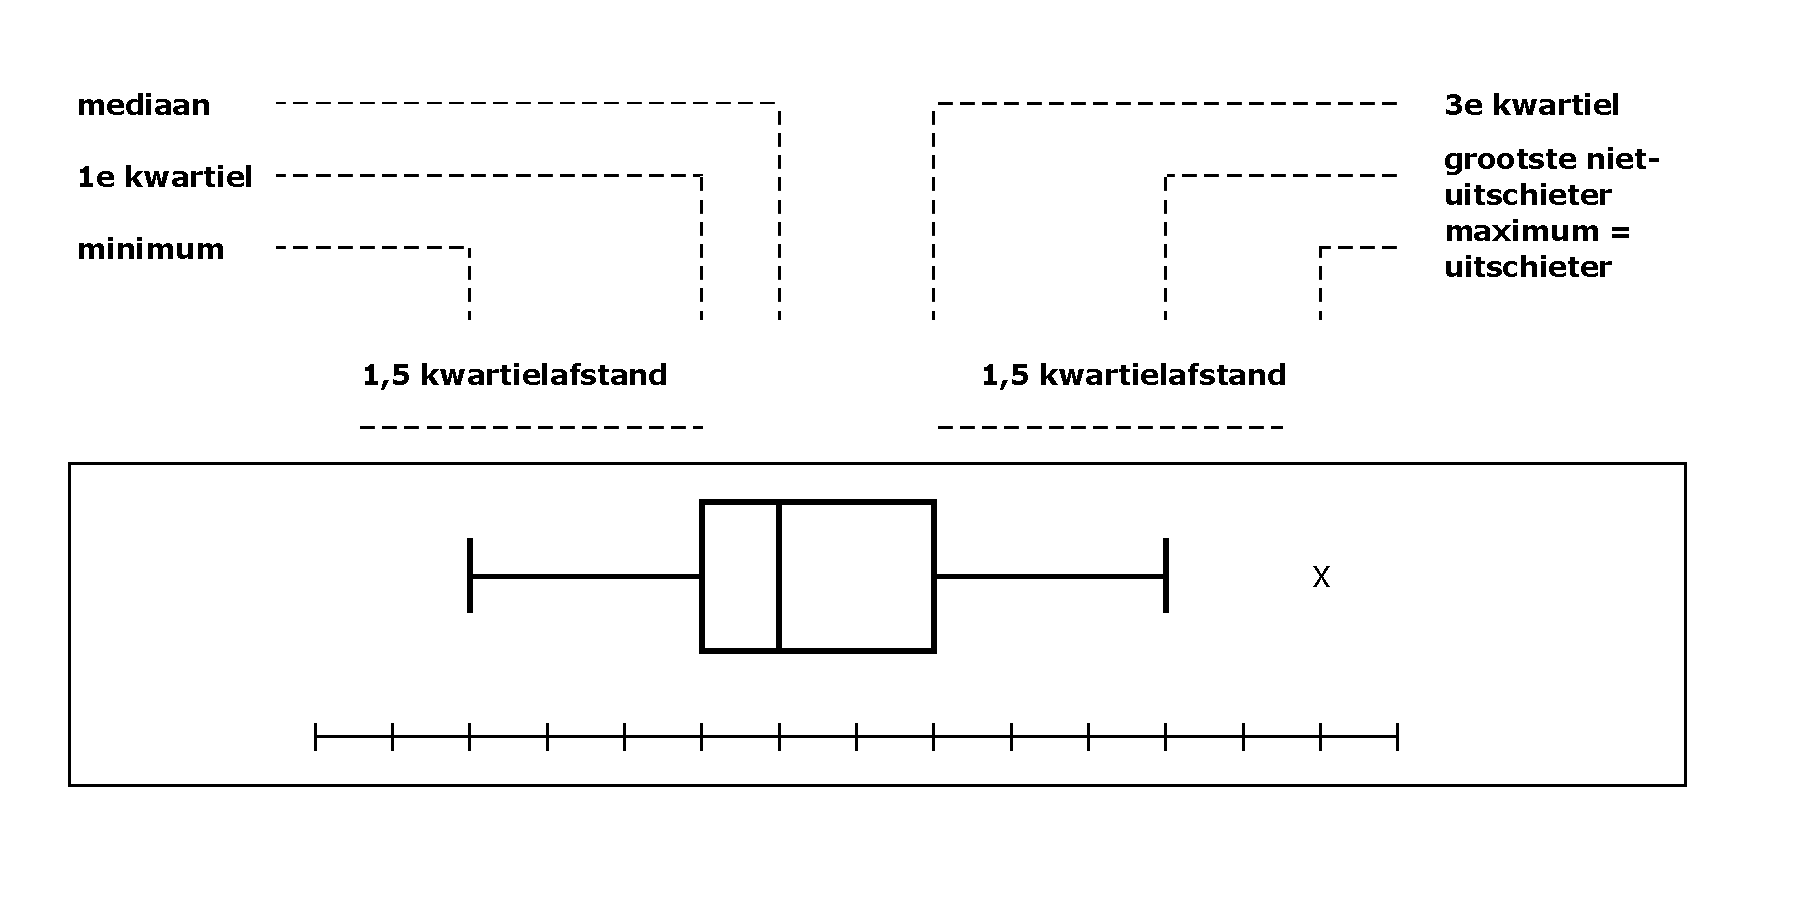
\includegraphics[width=\textwidth]{boxplot-schema}
\end{center}

\begin{oefening}
Een uitzendbureau onderzoekt bij haar ingeschreven studenten (dus allemaal studenten die effectief studentenjobs doen) hoeveel uur per jaar ze werken. Ze krijgen volgende dataset:

\dataset[10]{277, 356, 281, 32, 256, 281, 284, 332, 234, 262, 219, 235, 272, 141, 249, 282, 288, 306, 313, 82, 309, 284, 258, 329, 290, 316, 168, 255, 214, 293, 330, 258, 43, 244, 302, 214, 290, 223, 333, 265, 269, 255, 280, 271, 261, 327, 246, 245, 301, 325, 225, 275}

We vinden volgende kengetallen:
\begin{center}
  \begin{tabular}{r|l}
    Minimum & 32\\
    Eerste kwartiel & 244.5\\
    Mediaan & 271.5\\
    Derde kwartiel & 297\\
    Maximum & 356
  \end{tabular}
\end{center}

\begin{enumerate}[(a)]
  \item Controleer of de kengetallen kloppen.
  \item Hoeveel is $IQR$?
  \item Hoeveel is $Q_1-1.5\cdot IQR$
  \item Hoeveel is $Q_3+1.5\cdot IQR$
  \item Teken de boxplot.
\end{enumerate}
\end{oefening}

\cleardoublepage
\section{Extra oefeningen}

\begin{oefening}
Wanneer is een kwantitatieve variabele continu? Zeg dat in je eigen woorden, en geef
enkele voorbeelden.
\end{oefening}

\begin{oefening}
Schrijf je een continu kwantitatieve variabele altijd op met kommagetallen? Motiveer je
antwoord.
\end{oefening}

\begin{oefening}
Welke eigenschap probeert de standaardafwijking te beschrijven? Zeg in woorden hoe je de
standaardafwijking berekent. Kan je daaruit afleiden of de standaardafwijking gevoelig is
voor uitschieters? Kan je daarvan een eenvoudig voorbeeld geven?
\end{oefening}

\begin{oefening}
Welke eigenschap probeert de interkwartielafstand te beschrijven? Zeg in woorden wat
kwartielen zijn en hoe je de interkwartielafstand berekent. Kan je daaruit afleiden of de
interkwartielafstand gevoelig is voor uitschieters? Kan je daarvan een eenvoudig voorbeeld
geven?
\end{oefening}

\begin{oefening}
Geef de benaming of het symbool van volgende kengetallen en duidt aan, met een kruisje, of ze al dan niet centrummaten of spreidingsmaten zijn.\\
\begin{center}
  \begin{tabular}{c|c|c|c|c}
        & Kengetal        & Symbool     & Centrummaat & Spreidingsmaat \\
    \hline
    (a) & \arule{4cm}     & $\bar{x}$   & \arule{1cm} & \arule{1cm}    \\
    (b) & Mediaan         & \arule{2cm} & \arule{1cm} & \arule{1cm}    \\
    (c) & Variatiebreedte & \arule{2cm} & \arule{1cm} & \arule{1cm}    \\
    (d) & \arule{4cm}     & $IQR$       & \arule{1cm} & \arule{1cm}    \\
  \end{tabular}
\end{center}
\end{oefening}

\pagebreak
\section{Voorbeeld examenvragen}

\paragraph{Vraag 1}
Van de {\em sweet \& fair shop} krijg je de volgende dataset\footnote{Met dank aan de studenten van 6SETA.}:

druivensuiker aardbei; druivensuiker mango; kinderrozijnen; amandel chocolades; zure frieten; zure frieten; coco-mango reep; koban mix; kinderrozijnen; druivensuiker mango; zure frieten; kinderrozijnen;  druivensuiker mango; druivensuiker aardbei;  druivensuiker mango; druivensuiker mango; druivensuiker mango; druivensuiker aardbei; druivensuiker aardbei; druivensuiker aardbei; druivensuiker aardbei; kinderrozijnen;

Stel een frequentietabel op:
\begin{center}
  \begin{tabular}{p{4cm}|p{4cm}|p{4cm}}
    &absolute frequentie&relatieve frequentie\\
    \hline
    &&\\[6cm]
  \end{tabular}
\end{center}

Wat heb je genomen als variabele? \arulefill
Dit is een kwalitatieve/kwantitatieve variabele. {\tiny (schrappen wat niet past)}
Wat is de steekproefgrootte? \arulefill
Er zijn twee manieren om de data grafisch voor te stellen, welke:
\begin{itemize}
  \item \arule{6cm}
  \item \arule{6cm}
\end{itemize}

\newpage
Stel je data grafisch voor (op twee manieren)

\ruitjes{20cm}

\newpage
\paragraph{Vraag 2}
Aan een aantal studenten uit het eerste jaar hoger onderwijs werd gevraagd hoeveel auto's er bij hen in het gezin waren. De data die we terugkregen was als volgt:
2; 0; 3; 1; 1; 1; 3; 1; 1; 1; 2; 1; 0; 0; 2; 0; 0; 0; 7; 1; 2; 2; 2; 2; 1; 1; 1; 2; 2; 3

Wat zijn de elementen in dit onderzoek? \arulefill

Welke variabele wordt hier onderzocht? \arulefill

Waarom mag je zeggen dat de variabele in dit onderzoek kwantitatief is?
\arules{2}

Is de kwantitatieve variabele discreet of continue?
\arules{1}

Vervolledig de frequentietabel (het is niet nodig om de data in klassen op te delen):
\begin{center}
  \setlength{\tabcolsep}{7pt}
  \renewcommand{\arraystretch}{1.5}
  \begin{tabular}{p{4cm}|p{4cm}|p{4cm}}
      &    & \\
    \hline
    0 &    & \\
    1 &    & \\
    2 &    & \\
    3 &    & \\
    4 &    & \\
    5 &    & \\
    6 &    & \\
    7 &    & \\
      & n= & \\
  \end{tabular}
\end{center}

Maak een histogram waarin je absolute frequenties gebruikt.

\begin{center}
\definecolor{cqcqcq}{rgb}{0.65,0.65,0.65}
\begin{tikzpicture}[xscale=1,yscale=0.3,line cap=round,line join=round,>=triangle 45,x=1.0cm,y=1.0cm]
\draw [color=cqcqcq,dash pattern=on 1pt off 1pt, xstep=1.0cm,ystep=1.0cm] (-1,-1) grid (12,12);
\draw[->,color=black] (-1,0) -- (12,0);
\draw[shift={(1,0)},color=black] (0pt,2pt) -- (0pt,-2pt) node[below] {\footnotesize $1$};
\draw[color=black] (0.25,12.07) node [anchor=south west] { x};
\draw[->,color=black] (0,-1) -- (0,12);
\draw[shift={(0,1)},color=black] (2pt,0pt) -- (-2pt,0pt) node[left] {\footnotesize $1$};
\draw[color=black] (12.09,-1.25) node [anchor=west] { y};
\draw[color=black] (0pt,-10pt) node[right] {\footnotesize $0$};
\end{tikzpicture}
\end{center}

Is het belangrijk de grootste absolute frequentie vooraan wordt geplaatst?
\arules{1}

In hoeveel gezinnen zijn er $4$ auto's? \arulefill
Waarom staat de waarde $4$ dan toch in de frequentietabel?
\arules{2}

Is het nuttig om ook in het histogram een plaatsje op de $x$-as te voorzien voor $4$ auto's, hoewel er daar geen staaf getekend is?
\arules{2}

Bereken het gemiddeld aantal auto's per gezin:
%\vspace*{1cm}
$$\bar{x}=\arule{5cm}$$

Voor wat is het gemiddelde gevoelig? \arulefill

Wat is de oplossing hierop? \arulefill

Geef deze voor ons voorbeeld: \arulefill

\newpage
\paragraph{Vraag 3}
Tijdens de opendeurdag laat de afdeling hout de leerlingen uit het zesde leerjaar planken zagen op 180 cm. Na tien planken meten we de reeds gezaagde planken en we vinden de volgende lengtes:\\
177; 178; 178; 179; 179; 180; 181; 181; 183; 184 cm\\

{\em Bereken of bepaal m.b.v. \zrm{ZRM} en geef ook steeds het correcte symbool!}

Steekproefgrootte:\arulefill

Gemiddelde:\arulefill

Standaard afwijking\footnote{$s = \sqrt{\frac{\mbox{som van alle gekwadrateerde afwijkingen t.o.v. het gemiddelde}}{n-1}} = \sqrt{\frac{\sum_{i=0}^n(\bar{x}-x_i)^2}{n-1}}$}:\arulefill

Maximum:\arulefill

Minimum:\arulefill

Eerste kwartiel:\arulefill

Mediaan:\arulefill

Derde kwartiel:\arulefill

Interkwartielafstand:\arulefill

Teken de boxplot:

\ruitjes{3cm}

\end{document}
